\chapter{Architecture / Design du protocole}
\label{ch:arch}
Dans ce chapitre, je vais m'intéresser à expliquer le fonctionnement de la \textit{certificateless cryptography} et démontrer comment je l'ai utilisée afin de l'intégrer à un protocole de chiffrement de mail.
\section{Architecture globale}
Dans cette Figure \ref{fig:globalProtocol}, je présente uniquement l'architecture globale pour bien représenter les différents acteurs présents dans le protocole et ainsi avoir une vue d'ensemble pour faciliter la compréhension.
\begin{figure}[h!]
	\centering
	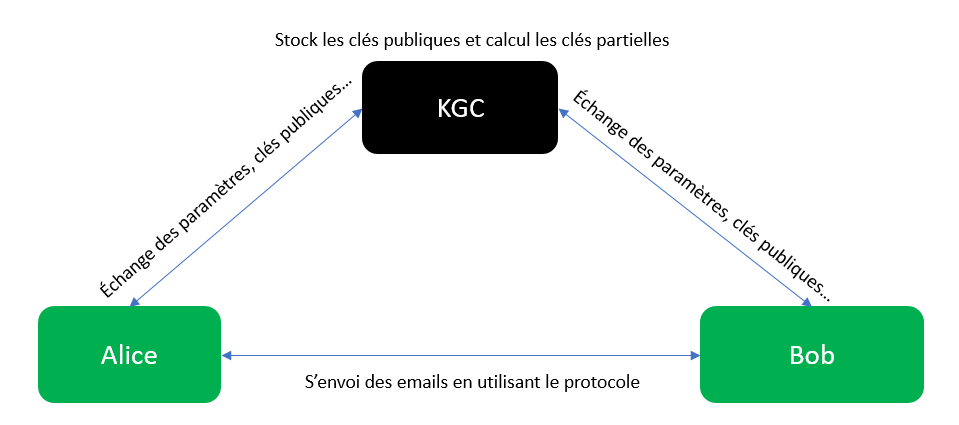
\includegraphics[width=14cm]{images/SchemaGlobal.png}
	\caption{Schéma global du protocole}
	\label{fig:globalProtocol}
\end{figure}
%TODO compléter ce chapitre et préciser les actions des acteurs plus en détails
\section{Acteurs}
Les parties impliquées sont les suivantes comme vu à la figure \ref{fig:globalProtocol}.
\begin{itemize}
	\item Alice : L'envoyeur du message de mail en direction de Bob, ainsi elle doit discuter avec le KGC.
	\item Bob : Le destinataire du message, communique uniquement avec le KGC en ayant reçu le message d'Alice.
	\item KGC : Permet aux différents acteurs de pouvoir récupérer les Public Keys des clients, mais aussi recevoir les Partial Private Keys. 
\end{itemize}
Ces partis sont les principaux présents dans un exemple de Certificateless Cryptography.
\section{Fonctionnement Certificateless PKC}
Je vais ici découper les différents algorithmes présent dans le certificateless public key cryptography. En passant par le chiffrement et la signature.
Ces algorithmes seront accompagnés d'explications sur leur utilité. Les noms donnés aux algorithmes seront réutilisés ensuite pour les schémas afin de démontrer l'architecture du protocole mis en place. L'on peut voir des définitions spécifiques dans l'article sur lequel je me suis appuyé pour ce travail~\cite{DBLP:conf/pkc/DentLP08}.
\subsection{Chiffrement}
Liste des différents algorithmes de \textit{Certificateless Cryptography} et leur description.
\begin{itemize}
	\item \textit{Setup.} (seulement une fois par le KGC).
	\item \textit{Partial-Private-Key-Extract.} Calcul d'une clé privée partielles lorsque qu'un client le demande pour identité donnée.
	\item \textit{Set-Secret-Value.} Le client ne le fait qu'une fois pour tirer sa valeur secrète.
	\item \textit{Set-Private-Key.} Le client combine ses clés partielles et sa clé secrète pour obtenir une clé privée afin de déchiffrer les message reçus, chiffrés avec une certaine identité.
	\item \textit{Set-Public-Key.} Le client ne le fait qu'une fois, il calcule sa clé publique en fonction de sa valeur secrète.
	\item \textit{Encrypt.} Chiffre un message avec la clé publique du destinataire et son identité.
	\item \textit{Decrypt.} Déchiffres un message utilisant sa clé privée et l'identité utilisée pendant le chiffrement.
\end{itemize}
\subsection{Signature}
Pour la signature les algorithmes sont les mêmes avec une différence dans leur conception et évidemment le \textit{Encrypt} et \textit{Decrypt} sont remplacé par \textit{Sign} et \textit{Verify}.
%TODO compléter voir tableau
Dans la littérature certificateless les schémas de signatures sont beaucoup plus cassés que ceux de chiffrement apparemment (voir tableau ). Il faut donc faire attention à suivre les schémas afin de vérifier que le schéma choisi ne soit pas mis à mal.
\section{Design du protocole}
%\begin{figure}[h!]
%	\centering
%	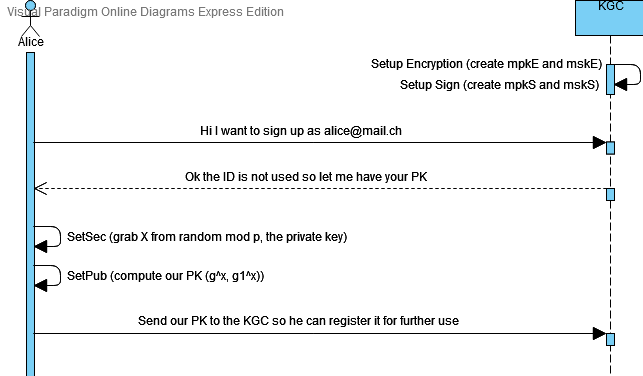
\includegraphics[width=14cm]{images/firstConnexion.png}
%	\caption{Schéma de la première connexion}
%	\label{fig:firstConn}
%\end{figure}
\begin{figure}
[h!]
	\centering
	\begin{sequencediagram}
		\newthread{A}{Alice}{}
		\newinst[10]{B}{KGC}{} 
		\begin{call}{A}{Initialisation with alice@mail.ch}{B}{OK, ID not in use. Give PK}
		\end{call}
	\postlevel
		\begin{callself}{A}{SetSec $x = Z_p$}{}
		\end{callself}
	\postlevel
		\begin{callself}{A}{SetPub $PK_{Alice} = (g^x, g_{1}^x)$}{}
		\end{callself}
	\postlevel
		\begin{call}{A}{$PK_{Alice}$}{B}{}
		\end{call}
		
	\end{sequencediagram}
	\caption{Schéma de la première connexion}
	\label{fig:firstConn}
\end{figure}

Dans la Figure \ref{fig:firstConn} l'on voit la première connexion d'un utilisateur mais aussi le Setup du serveur, cette étape ne se fera qu'une fois dans la vie du KGC. Mais le Setup doit tout de même être fait pour la partie de signature et la partie de chiffrement.
Ensuite Alice veut s'enregistrer auprès du KGC, ainsi le KGC lui renvoi les paramètres publiques (mpkS et mpkE) si aucun utilisateur n'a déjà cet email.
L'utilisateur va alors crée sa valeur secrète tirée aléatoire modulo p puis générer sa clé publique.
Pour finir Alice envoi sa clé publique au KGC afin qu'il l'associe à son ID et puisses le donner aux personnes qui veulent envoyer un mail à Alice.\\

%\begin{figure}[h!]
	%\centering
	%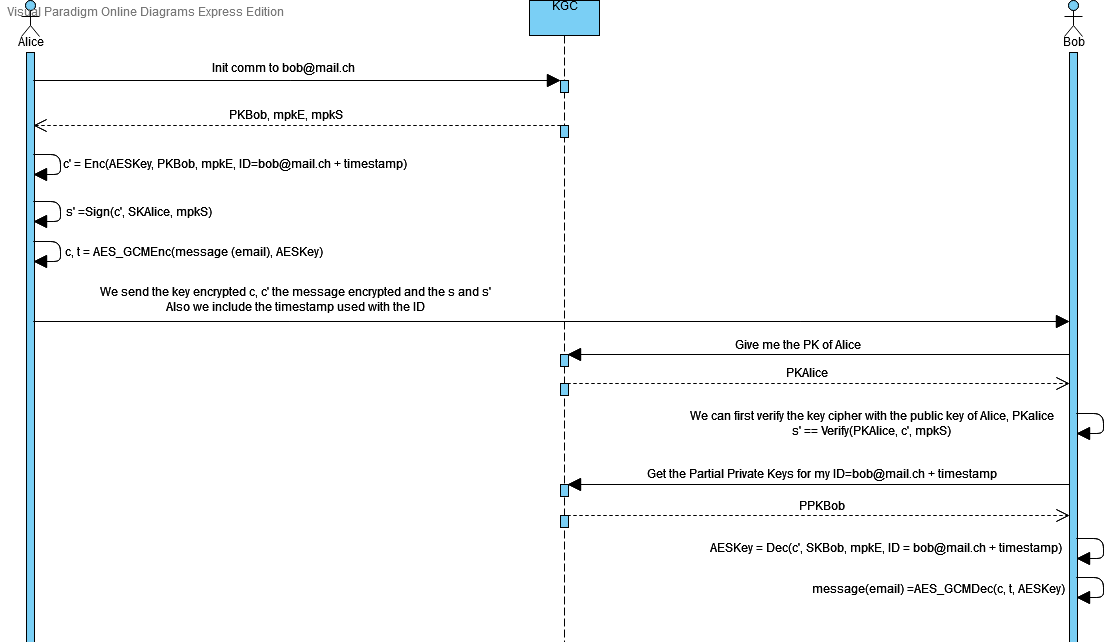
\includegraphics[width=14cm]{images/aliceSendsToBob.png}
	%\caption{Alice envoi un message à Bob}
	%\label{fig:aliceSends}
%\end{figure}

\begin{figure}
[h!]
	\centering
	\begin{sequencediagram}
		\newthread{A}{Alice}{}
		\newinst[9]{B}{KGC}{} 
		\newinst[3]{C}{Bob}{}
		\begin{call}{A}{Comm. with bob@mail.ch}{B}{$PKE_{Bob} $}
		\end{call}
		\postlevel
		\begin{call}{A}{Extract alice@mail.ch + time}{B}{$PPKS_{Alice}$}
		\end{call}
		\postlevel
		\begin{callself}{A}{$c'  = ENC_{PKE_{Bob}}(AES_K, bob@mail.ch + time)$}{}
		\end{callself}
		\postlevel
		%TODO : mettre algo private keys signature
		\begin{callself}{A}{SetPrivSig $SKS_{Alice}' = $}{}
		\end{callself}
		\postlevel
		\begin{callself}{A}{$s' = Sign(c', SKS_{Alice})$}{}
		\end{callself}
		\postlevel
		\begin{callself}{A}{$c, t = AESGCM_{AESK}(mesage)$}{}
		\end{callself}
		\postlevel
		\begin{call}{A}{time, c', c, t, s', IV}{C}{}
		\end{call}
	\end{sequencediagram}
	\caption{Alice envoit un message à Bob}
	\label{fig:aliceSends}
\end{figure}

Dans la Figure \ref{fig:aliceSends} l'on voit comment se déroulerait l'envoi d'un message à Bob : 
\begin{itemize}
	\item Tout d'abord, Alice va récupérer le clé publique de Bob via son ID (aka email).
	\item Elle devra aussi récupérer sa clé privée partielle de signature pour créer ses clés privées afin de signer le message. Elle va le faire à l'aide de son ID et du même timestamp qu'utilisé pour la suite.
	\item Elle va ensuite tirer une valeur aléatoire dans Gt qui représentera sa clé AES pour la suite, elle va chiffrer cet élément à l'aide de la clé publique de Bob et de son ID complété par un timestamp. Ce timestamp sert à garder une certaine Forward Secrecy. Le cipher sera c'.
	\item Elle va calculer la signature du cipher donné (s' sur la figure)
	\item Alice utilisera un chiffrement authentifié comme AES\_GCM pour chiffrer et authentifié son mail à Bob, t pour le tag et c pour le cipher.
	\item Finalement elle va envoyer tout ces éléments à bob (à savoir, l'ID utilisé, c, c', t, s' et l'IV utilisé pour AES\_GCM).
\end{itemize}

\begin{figure}
[h!]
	\centering
	\begin{sequencediagram}
		\newthread{A}{Bob}{}
		\newinst[9]{B}{KGC}{} 
		\newinst[3]{C}{Alice}{}
		\begin{messcall}{C}{time, c', c, t, s', IV}{A}
		\end{messcall}
		\postlevel
		\begin{call}{A}{PK of alice@mail.ch}{B}{$PK_{Alice}$}
		\end{call}
		\postlevel
		\begin{callself}{A}{$s' == Verify(c', PK_{Alice})$}{}
		\end{callself}
		\postlevel
		\begin{call}{A}{Extract bob@mail.ch + time}{B}{$PPKE_{Bob}$}
		\end{call}
		\postlevel
		\begin{callself}{A}{SetPriv $SKE_{Bob}' = $}{}
		\end{callself}
		\postlevel
		\begin{callself}{A}{$AES_K = DEC_{SKE_{Bob}}(c', ID=bob@mail.ch+time)$}{}
		\end{callself}
		\postlevel
		\begin{callself}{A}{$message = AESGCM_{AES_K}(c,t, IV)$}{}
		\end{callself}
	\end{sequencediagram}
	\caption{Bob reçoit le message}
	\label{fig:bobReceives}
\end{figure}

Mais dans la Figure \ref{fig:bobReceives} l'on voit comment la réception du côté de Bob se déroulerait :
\begin{itemize}
	\item A la réception la première chose à faire et de vérifier le cipher de la clé AES. Pour cela l'on va demander la clé publique d'Alice au KGC. Puis on va vérifier ce cipher c' à l'aide de sa signature s'.
	\item Ensuite Bob va récupérer sa clé privée partielle via le KGC en fournissant son ID avec le timestamp envoyé par Alice. Il va ainsi pouvoir former sa clé privée.
	\item Avec s clé privée il va pouvoir déchiffrer c' et obtenir la clé AES pour la suite.
	\item Une fois que l'on a la clé AES l'on peut simplement déchiffrer à l'aide d'AES\_GCM c pour obtenir le message initial.
\end{itemize}
